% Options for packages loaded elsewhere
\PassOptionsToPackage{unicode}{hyperref}
\PassOptionsToPackage{hyphens}{url}
\PassOptionsToPackage{dvipsnames,svgnames,x11names}{xcolor}
%
\documentclass[
  letterpaper,
  DIV=11,
  numbers=noendperiod]{scrartcl}

\usepackage{amsmath,amssymb}
\usepackage{iftex}
\ifPDFTeX
  \usepackage[T1]{fontenc}
  \usepackage[utf8]{inputenc}
  \usepackage{textcomp} % provide euro and other symbols
\else % if luatex or xetex
  \usepackage{unicode-math}
  \defaultfontfeatures{Scale=MatchLowercase}
  \defaultfontfeatures[\rmfamily]{Ligatures=TeX,Scale=1}
\fi
\usepackage{lmodern}
\ifPDFTeX\else  
    % xetex/luatex font selection
  \setmainfont[]{IBM Plex Sans}
\fi
% Use upquote if available, for straight quotes in verbatim environments
\IfFileExists{upquote.sty}{\usepackage{upquote}}{}
\IfFileExists{microtype.sty}{% use microtype if available
  \usepackage[]{microtype}
  \UseMicrotypeSet[protrusion]{basicmath} % disable protrusion for tt fonts
}{}
\makeatletter
\@ifundefined{KOMAClassName}{% if non-KOMA class
  \IfFileExists{parskip.sty}{%
    \usepackage{parskip}
  }{% else
    \setlength{\parindent}{0pt}
    \setlength{\parskip}{6pt plus 2pt minus 1pt}}
}{% if KOMA class
  \KOMAoptions{parskip=half}}
\makeatother
\usepackage{xcolor}
\setlength{\emergencystretch}{3em} % prevent overfull lines
\setcounter{secnumdepth}{5}
% Make \paragraph and \subparagraph free-standing
\ifx\paragraph\undefined\else
  \let\oldparagraph\paragraph
  \renewcommand{\paragraph}[1]{\oldparagraph{#1}\mbox{}}
\fi
\ifx\subparagraph\undefined\else
  \let\oldsubparagraph\subparagraph
  \renewcommand{\subparagraph}[1]{\oldsubparagraph{#1}\mbox{}}
\fi

\usepackage{color}
\usepackage{fancyvrb}
\newcommand{\VerbBar}{|}
\newcommand{\VERB}{\Verb[commandchars=\\\{\}]}
\DefineVerbatimEnvironment{Highlighting}{Verbatim}{commandchars=\\\{\}}
% Add ',fontsize=\small' for more characters per line
\usepackage{framed}
\definecolor{shadecolor}{RGB}{241,243,245}
\newenvironment{Shaded}{\begin{snugshade}}{\end{snugshade}}
\newcommand{\AlertTok}[1]{\textcolor[rgb]{0.68,0.00,0.00}{#1}}
\newcommand{\AnnotationTok}[1]{\textcolor[rgb]{0.37,0.37,0.37}{#1}}
\newcommand{\AttributeTok}[1]{\textcolor[rgb]{0.40,0.45,0.13}{#1}}
\newcommand{\BaseNTok}[1]{\textcolor[rgb]{0.68,0.00,0.00}{#1}}
\newcommand{\BuiltInTok}[1]{\textcolor[rgb]{0.00,0.23,0.31}{#1}}
\newcommand{\CharTok}[1]{\textcolor[rgb]{0.13,0.47,0.30}{#1}}
\newcommand{\CommentTok}[1]{\textcolor[rgb]{0.37,0.37,0.37}{#1}}
\newcommand{\CommentVarTok}[1]{\textcolor[rgb]{0.37,0.37,0.37}{\textit{#1}}}
\newcommand{\ConstantTok}[1]{\textcolor[rgb]{0.56,0.35,0.01}{#1}}
\newcommand{\ControlFlowTok}[1]{\textcolor[rgb]{0.00,0.23,0.31}{#1}}
\newcommand{\DataTypeTok}[1]{\textcolor[rgb]{0.68,0.00,0.00}{#1}}
\newcommand{\DecValTok}[1]{\textcolor[rgb]{0.68,0.00,0.00}{#1}}
\newcommand{\DocumentationTok}[1]{\textcolor[rgb]{0.37,0.37,0.37}{\textit{#1}}}
\newcommand{\ErrorTok}[1]{\textcolor[rgb]{0.68,0.00,0.00}{#1}}
\newcommand{\ExtensionTok}[1]{\textcolor[rgb]{0.00,0.23,0.31}{#1}}
\newcommand{\FloatTok}[1]{\textcolor[rgb]{0.68,0.00,0.00}{#1}}
\newcommand{\FunctionTok}[1]{\textcolor[rgb]{0.28,0.35,0.67}{#1}}
\newcommand{\ImportTok}[1]{\textcolor[rgb]{0.00,0.46,0.62}{#1}}
\newcommand{\InformationTok}[1]{\textcolor[rgb]{0.37,0.37,0.37}{#1}}
\newcommand{\KeywordTok}[1]{\textcolor[rgb]{0.00,0.23,0.31}{#1}}
\newcommand{\NormalTok}[1]{\textcolor[rgb]{0.00,0.23,0.31}{#1}}
\newcommand{\OperatorTok}[1]{\textcolor[rgb]{0.37,0.37,0.37}{#1}}
\newcommand{\OtherTok}[1]{\textcolor[rgb]{0.00,0.23,0.31}{#1}}
\newcommand{\PreprocessorTok}[1]{\textcolor[rgb]{0.68,0.00,0.00}{#1}}
\newcommand{\RegionMarkerTok}[1]{\textcolor[rgb]{0.00,0.23,0.31}{#1}}
\newcommand{\SpecialCharTok}[1]{\textcolor[rgb]{0.37,0.37,0.37}{#1}}
\newcommand{\SpecialStringTok}[1]{\textcolor[rgb]{0.13,0.47,0.30}{#1}}
\newcommand{\StringTok}[1]{\textcolor[rgb]{0.13,0.47,0.30}{#1}}
\newcommand{\VariableTok}[1]{\textcolor[rgb]{0.07,0.07,0.07}{#1}}
\newcommand{\VerbatimStringTok}[1]{\textcolor[rgb]{0.13,0.47,0.30}{#1}}
\newcommand{\WarningTok}[1]{\textcolor[rgb]{0.37,0.37,0.37}{\textit{#1}}}

\providecommand{\tightlist}{%
  \setlength{\itemsep}{0pt}\setlength{\parskip}{0pt}}\usepackage{longtable,booktabs,array}
\usepackage{calc} % for calculating minipage widths
% Correct order of tables after \paragraph or \subparagraph
\usepackage{etoolbox}
\makeatletter
\patchcmd\longtable{\par}{\if@noskipsec\mbox{}\fi\par}{}{}
\makeatother
% Allow footnotes in longtable head/foot
\IfFileExists{footnotehyper.sty}{\usepackage{footnotehyper}}{\usepackage{footnote}}
\makesavenoteenv{longtable}
\usepackage{graphicx}
\makeatletter
\def\maxwidth{\ifdim\Gin@nat@width>\linewidth\linewidth\else\Gin@nat@width\fi}
\def\maxheight{\ifdim\Gin@nat@height>\textheight\textheight\else\Gin@nat@height\fi}
\makeatother
% Scale images if necessary, so that they will not overflow the page
% margins by default, and it is still possible to overwrite the defaults
% using explicit options in \includegraphics[width, height, ...]{}
\setkeys{Gin}{width=\maxwidth,height=\maxheight,keepaspectratio}
% Set default figure placement to htbp
\makeatletter
\def\fps@figure{htbp}
\makeatother

\KOMAoption{captions}{tableheading}
\makeatletter
\makeatother
\makeatletter
\makeatother
\makeatletter
\@ifpackageloaded{caption}{}{\usepackage{caption}}
\AtBeginDocument{%
\ifdefined\contentsname
  \renewcommand*\contentsname{Table of contents}
\else
  \newcommand\contentsname{Table of contents}
\fi
\ifdefined\listfigurename
  \renewcommand*\listfigurename{List of Figures}
\else
  \newcommand\listfigurename{List of Figures}
\fi
\ifdefined\listtablename
  \renewcommand*\listtablename{List of Tables}
\else
  \newcommand\listtablename{List of Tables}
\fi
\ifdefined\figurename
  \renewcommand*\figurename{Figure}
\else
  \newcommand\figurename{Figure}
\fi
\ifdefined\tablename
  \renewcommand*\tablename{Table}
\else
  \newcommand\tablename{Table}
\fi
}
\@ifpackageloaded{float}{}{\usepackage{float}}
\floatstyle{ruled}
\@ifundefined{c@chapter}{\newfloat{codelisting}{h}{lop}}{\newfloat{codelisting}{h}{lop}[chapter]}
\floatname{codelisting}{Listing}
\newcommand*\listoflistings{\listof{codelisting}{List of Listings}}
\makeatother
\makeatletter
\@ifpackageloaded{caption}{}{\usepackage{caption}}
\@ifpackageloaded{subcaption}{}{\usepackage{subcaption}}
\makeatother
\makeatletter
\@ifpackageloaded{tcolorbox}{}{\usepackage[skins,breakable]{tcolorbox}}
\makeatother
\makeatletter
\@ifundefined{shadecolor}{\definecolor{shadecolor}{rgb}{.97, .97, .97}}
\makeatother
\makeatletter
\makeatother
\makeatletter
\makeatother
\ifLuaTeX
  \usepackage{selnolig}  % disable illegal ligatures
\fi
\IfFileExists{bookmark.sty}{\usepackage{bookmark}}{\usepackage{hyperref}}
\IfFileExists{xurl.sty}{\usepackage{xurl}}{} % add URL line breaks if available
\urlstyle{same} % disable monospaced font for URLs
\hypersetup{
  colorlinks=true,
  linkcolor={blue},
  filecolor={Maroon},
  citecolor={Blue},
  urlcolor={Blue},
  pdfcreator={LaTeX via pandoc}}

\author{}
\date{}

\begin{document}
\ifdefined\Shaded\renewenvironment{Shaded}{\begin{tcolorbox}[frame hidden, boxrule=0pt, interior hidden, borderline west={3pt}{0pt}{shadecolor}, sharp corners, enhanced, breakable]}{\end{tcolorbox}}\fi

\renewcommand*\contentsname{Table of contents}
{
\hypersetup{linkcolor=}
\setcounter{tocdepth}{3}
\tableofcontents
}
\hypertarget{managing-code-page-conversion}{%
\section{Managing code page
conversion}\label{managing-code-page-conversion}}

\hypertarget{introduction}{%
\subsection{Introduction}\label{introduction}}

Choosing Git to host enterprise-level software assets implies a
migration task of the z/OS artifacts. Whether the source code is under
the control of a legacy SCM solution or not, these artifacts are
typically stored as members within partitioned data sets (PDSs) with a
specific encoding. Depending on locale, country languages, regulations
or work habits, the encoding of the source code can differ by various
specificities such as accents, locale typography and characters. To
support these peculiarities, many different EBCDIC code pages were
developed in z/OS and are now widely used.

In the Git world, the standard prevailing encoding is UTF-8, which
supports most (if not all) of the characters used in printing worldwide.
When migrating artifacts from z/OS to Git, a translation must occur to
convert the EBCDIC-encoded content of source files to UTF-8. This
process is transparent to the user, whereby the translation is performed
by the Rocket Git client, as long as the necessary information on how to
perform the conversion is provided. Git uses a specific file called
\texttt{.gitattributes} to describe and dictate the translation
behavior. This page contains details on the encoding that should be used
when hosting the artifacts on z/OS or on Git repositories.

This page will highlight some specific migration situations and some
cautionary commentary that must be taken into account in order to ensure
a successful migration of z/OS artifacts to Git. The purpose of this
document is not to cover all the country-related specificities, nor the
complex encodings found worldwide. Rather it is aimed at presenting
general use cases and how to prevent/circumvent potential pitfalls.

\hypertarget{understanding-the-code-page-translation-process}{%
\subsection{Understanding the code page translation
process}\label{understanding-the-code-page-translation-process}}

Code page translation has always been a challenge since z/OS is
exchanging data with the distributed systems. To completely understand
the effect of encoding, it is important to take a step back and analyze
the binary content of files. This analysis will help to better visualize
the transformation process that is occurring behind the scenes

\hypertarget{looking-inside-a-file}{%
\subsubsection{Looking inside a file}\label{looking-inside-a-file}}

A file itself can be summarized as being a series of bytes, often
expressed in the hexadecimal notation (from x'00' to x'FF'). This file
can represent binary content which is not meant to be human-readable
(like an executable file), or text content. For the latter and from a
user standpoint, this series of bytes doesn't mean anything if the
content is not associated with a code page, which will link each byte to
a printable character (or a control character). Printable characters are
the formation of a character set.

The combination of the contents of a file and the code page used defines
the human-readable content. That said, the contents of a file will be
displayed slightly differently when combined with different code pages.
Let's explore a couple of examples using the ISPF Editor with the ``HEX
VERT'' option enabled to show the hexadecimal values of a file.

Consider the following example where a file containing the French
sentence ``Bonjour à tous !'' (which translates to ``Hello everyone!'')
is displayed with two different code pages. The file which contains this
sentence was saved using IBM-1147 encoding. When the file is then
displayed using a different encoding of IBM-1047, although the contents
of the file is the same from a binary standpoint, some characters are
displayed in a different way:

\begin{itemize}
\item
  Using the IBM-1147 code page:

  \begin{figure}

  {\centering 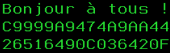
\includegraphics{static/img/bonjour-ibm-1147.png}

  }

  \caption{Using the IBM-1147 code page}

  \end{figure}
\item
  Using the IBM-1047 code page:

  \begin{figure}

  {\centering 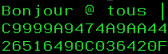
\includegraphics{static/img/bonjour-ibm-1047.png}

  }

  \caption{Using the IBM-1047 code page}

  \end{figure}
\end{itemize}

To be correctly displayed with the IBM-1047 code page, the contents of
this file must be transformed. Please note how the hexadecimal codes for
the \texttt{à} and the \texttt{!} characters changed, respectively from
x'7C' to x'44' and from x'4F' to x'5A':

\begin{itemize}
\item
  Transforming to the IBM-1047 code page:

  \begin{figure}

  {\centering 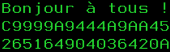
\includegraphics{static/img/bonjour-transform.png}

  }

  \caption{Transforming to the IBM-1047 code page}

  \end{figure}
\end{itemize}

It is important to understand that the code page plays a determining
role not only when displaying a file, but also when editing it. To
ensure the content of a file is consistent when used by different
people, the code page used for editing and displaying will likely be the
same for all the users. If Alice edits a file with the IBM-1147 code
page and introduces characters (like accents) specific to that code
page, then Bob will need to use the IBM-1147 code page to display the
content of this file. Otherwise, he may experience the situation
depicted earlier, where accents are not displayed correctly. If Bob uses
the IBM-1047 code page to edit the file and change the content to
replace the special characters by the corresponding accents, then Alice
will not be able to display the content of this file like she entered it
on her terminal.

Consider this next example. A program file, such as C/370, employs the
left (\texttt{{[}}) and right (\texttt{{]}}) brackets in some of the
language statement constructs. In many US-based legacy applications, the
original encoding used to create source files was IBM-037. If these
files are then displayed using a different encoding of IBM-1047, again,
although the content of the files is the same from a binary standpoint,
the brackets are not displayed the correct way:

\begin{itemize}
\item
  Using the IBM-037 code page:

  \begin{figure}

  {\centering 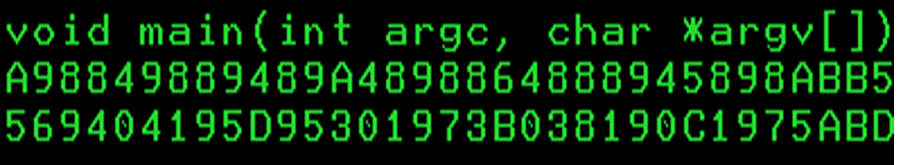
\includegraphics{static/img/void-main-ibm-037.png}

  }

  \caption{Using the IBM-1147 code page}

  \end{figure}
\item
  Using the IBM-1047 code page:

  \begin{figure}

  {\centering 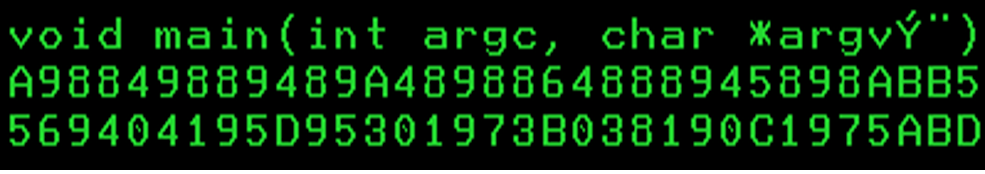
\includegraphics{static/img/void-main-ibm-1047.png}

  }

  \caption{Using the IBM-1047 code page}

  \end{figure}
\end{itemize}

To be correctly displayed with the IBM-1047 code page, the contents of
this file must be transformed. The hexadecimal codes for the
\texttt{{[}} and the \texttt{{]}} characters must be changed from x'BA'
and x'BB' to x'AD' and x'BD', respectively:

\begin{itemize}
\item
  Transforming to the IBM-1047 code page:

  \begin{figure}

  {\centering 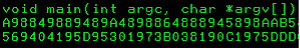
\includegraphics{static/img/void-main-transform.png}

  }

  \caption{Transforming to the IBM-1047 code page}

  \end{figure}
\end{itemize}

Again, it is very important that anyone and everyone who displays or
edits the file uses a consistent code page. This can sometimes be a
challenge, as the code page to be used is generally specified in the
3270 Emulator (TN3270) client session set-up. Another challenge is
trying to determine the original encoding used to create the file.

To summarize, the binary content of a file must be transformed to ensure
consistency when displayed with another code page. This process is known
as the code page translation and is key when migrating your source from
your z/OS platform to a distributed platform, which is using different
code pages (and most likely today, UTF-8).

\hypertarget{vocabulary}{%
\subsubsection{Vocabulary}\label{vocabulary}}

In this document, we will interchangeably use the coded character set ID
(CCSID), its equivalent name, and the code page to designate an
encoding. Although not strictly equivalent, they are all often
interchanged for the sake of convenience. For instance, the IBM-1047
code page is equivalent to the 1047 coded character set (CCSID) and is
usually named IBM-1047. The code page for IBM-037 is equivalent to coded
character set (CCSID) 037 and is usually named IBM-037. The CCSID for
UTF-8 is 1208 and is linked with many code pages.

To simplify, the code pages will be designated by their
\href{https://www.ibm.com/docs/en/zos-connect/zosconnect/3.0?topic=properties-coded-character-set-identifiers}{common
name}, for instance IBM-037, IBM-1047, IBM-1147, and UTF-8.

For reference, a list of code pages is available in the
\href{https://www.ibm.com/docs/en/personal-communications/14.0?topic=SSEQ5Y_14.0.0/com.ibm.pcomm.doc/reference/html/hcp_referencet002.htm}{Personal
Communications documentation site}.

\hypertarget{the-challenge-of-migrating-to-utf-8}{%
\subsubsection{The challenge of migrating to
UTF-8}\label{the-challenge-of-migrating-to-utf-8}}

If you have ever tried transferring a z/OS data set to a distributed
machine running a traditional operating system (like Microsoft Windows
or Linux), you probably ended up with similar content when opening the
file:

\begin{figure}

{\centering 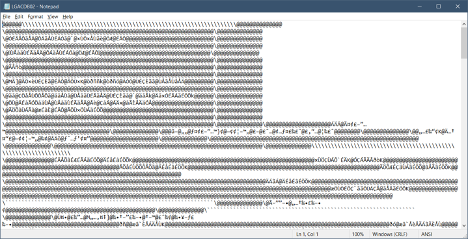
\includegraphics{static/img/unreadable.png}

}

\caption{Unreadable file due to transfer without code page conversion}

\end{figure}

The content is unreadable because the transfer was performed without a
code page conversion. This generally happens when the file was
transferred as binary, which leaves the content of the file untouched.
Most of the transfer utilities offer the capability to transfer the
files as binary or as text. In the latter option, code page conversion
occurs, and the file should be readable on distributed platforms.

The same conversion must be performed for text files when migrating to
Git. Generally, Git uses the UTF-8 code page and, as such, a translation
must occur on the content of the transferred files. Likewise, when
bringing the files back from Git to z/OS, a backward conversion must be
performed to ensure the files are correctly read with the code page in
use. Failure in performing this conversion may break the contents of the
files, which could become damaged and unreadable. Recovering from this
failure is difficult, and the best solution is usually to restart the
conversion all over again from the beginning, which often means deleting
the files in Git and transferring the same files from z/OS again.

\hypertarget{managing-non-printable-and-non-roundtripable-characters}{%
\subsubsection{Managing non-printable and non-roundtripable
characters}\label{managing-non-printable-and-non-roundtripable-characters}}

In the traditional EBCDIC code pages, some characters exist to control
the different devices themselves or the way text should be displayed.
These characters are located in the first 64 positions of the
\href{https://en.wikipedia.org/wiki/EBCDIC\#Definitions_of_non-ASCII_EBCDIC_controls}{EBCDIC
characters tables} and can be classified into 2 categories: the
non-printable characters and the non-roundtripable characters.

\begin{itemize}
\tightlist
\item
  Non-printable characters: These characters can be translated from
  EBCDIC to UTF-8 and back to EBCDIC without breaking the content of the
  file. However, editing files which contain these characters with
  editing tools on a distributed platform, can cause display issues.
  Non-printable characters include all EBCDIC characters below 0x40.
\item
  Non-roundtripable characters: The translation is still possible from
  EBCDIC to UTF-8, but the translation back to EBCDIC is not possible.
  In this case, the translated file is no longer identical to its
  original version. This specific situation must be considered and
  managed prior to the migration to Git. For these special characters,
  the conversion from EBCDIC to UTF-8 is generally feasible, but the
  resulting content of the files may be scrambled or displayed in a
  wrong way. Moreover, when transferring the files back to z/OS, the
  files could be damaged, and the transfer could even fail.
  Non-roundtripable characters include the following:

  \begin{itemize}
  \tightlist
  \item
    EBCDIC

    \begin{itemize}
    \tightlist
    \item
      Newline: 0x15
    \item
      Carriage return: 0x0D
    \item
      Line feed: 0x25
    \item
      SHIFT\_IN/SHIFT\_OUT: 0x0F \& 0x0E
    \end{itemize}
  \end{itemize}
\end{itemize}

In a migration process, when either non-printable or non-roundtripable
characters are found, two options are presented:

\begin{itemize}
\tightlist
\item
  Keep these characters ``as-is'' with the risk of damaging the source
  files.
\item
  Modify the characters to a conversion-friendly format.
\end{itemize}

For the first option, it is possible to keep the content of the files
intact, but the cost of this is to manage the file as a binary artifact
in Git. The benefit of this configuration is that the content of the
file is not altered by Git when the file is transferred. Because it is
flagged as binary, the contents are not converted to UTF-8 and remain
the same across the entire workflow (that is, from z/OS PDS to Git to
z/OS PDS). The major drawback of this method is that the modification of
these binary files with a distributed platform tool, such as an
integrated development environment (IDE) or Notepad, will be extremely
difficult. As these files were not converted to UTF-8, their contents
will still be in EBCDIC, which is rarely supported outside of the z/OS
platform. Browsing or editing the content of these files would require
to bring them back to the z/OS platform. Still, this option could be a
valid strategy for files that rarely (or never) change, but this implies
setting up a strategy when a modification is required (that is, these
files will need to be modified on z/OS, not using a distributed solution
- this strategy should remain as an exception).

The alternative is to opt for a transformation of the content that
contains non-printable or non-roundtripable characters before migrating
the files. Programmers have often employed elaborate strategies based on
the use of these characters in literals or constants. Through the ISPF
editor, developers have been able to insert hexadecimal values (when
enabling the editing of raw data with the hex on feature) in their
source code. This use case is very common and can easily be corrected by
replacing the hexadecimal coded characters with their corresponding
hexadecimal values as shown in the picture below (taken from a CICS
COBOL copybook):

\begin{itemize}
\item
  Initial values:

  \begin{figure}

  {\centering 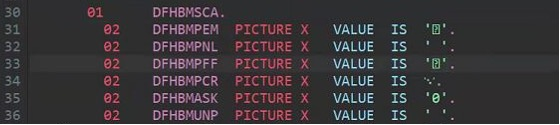
\includegraphics{static/img/code-page-initial-values.jpg}

  }

  \caption{Initial values}

  \end{figure}
\item
  Final values after transformation:

  \begin{figure}

  {\centering 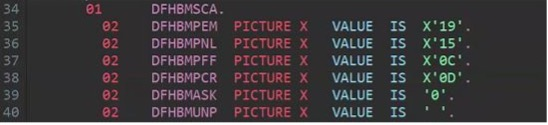
\includegraphics{static/img/code-page-values-after-transformation.jpg}

  }

  \caption{Final values after transformation}

  \end{figure}
\end{itemize}

This transformation could even be automated (albeit cautiously) through
scripting. Other use cases for these characters should be analyzed
carefully, and developers should be encouraged to write their source
code in a way that allows for code page conversion.

Fortunately, IBM Dependency Based Build (DBB) provides a feature in its
migration script to detect these special characters and helps manage
their code page conversion or their transfer as binary.

In any case, the decision about using binary-tagged files in Git,
refactoring these files to transform the non-printable and
non-roundtripable characters into their hex values, or not changing the
content of the files should be taken prior to performing the final
migration from datasets to Git repositories. If the migration is started
with files that contain either non-printable or non-roundtripable
characters, there is a high risk that files cannot be edited using
distributed editors. Once the files are migrated, it is often very
difficult to resolve the situation after the fact, as there can be
information lost during the code page conversion. In that situation, the
best option is to restart the migration from datasets, assuming the
original members are still available until the migration is validated.

\hypertarget{defining-the-code-page-of-files-in-git}{%
\subsection{Defining the code page of files in
Git}\label{defining-the-code-page-of-files-in-git}}

Since Git is a distributed system, each member of this ``network''
should be able to work with the files stored in the Git repositories.
Over the last decade, Git has become the de facto standard for the
development community, being used in all-sized enterprises, internal,
open-source and/or personal development projects. Because Git emerged in
the distributed world, it was first designed to support technologies
from this ecosystem, and it all started with the file encoding. Although
it appeared in the 90's, UTF-8 only gained notoriety in the 2010's
through the increased interconnectivity between heterogeneous systems.
UTF-8 is now recognized as the universal, common language for exchanging
data and files. Naturally, UTF-8 also became the standard for encoding
source files for the distributed world.

Since mainframe source resides on the host side under the control of a
Source Code Management solution, this source is encoded with an EBCDIC
code page and could potentially contain national characters. In order to
store these source files in Git, a code page conversion must occur
between the z/OS source file EBCDIC code page and UTF-8. This is the
role of the Rocket Git client on z/OS to perform that conversion, which
is transparent for the developers.

However, the Rocket Git client on z/OS must be instructed on the
conversion operation to perform. These instructions are defined in a
specific file that belongs to the Git repository. The
\href{https://www.git-scm.com/docs/gitattributes}{\texttt{.gitattributes}}
file is a standard file used by Git to declare specific attributes for
the Git Repository that it belongs to. With the Rocket Git client on
z/OS, it has been extended to describe the code page that should be used
for files when they are stored in Git and on z/OS UNIX System Services
(z/OS UNIX).

The structure of the file is straightforward. One or several attributes
are associated to each path and file extension listed in the file.
Wildcards can be used for generic definitions. This file must be encoded
in ASCII (ISO-8859-1), as it is processed by Git on z/OS and other Git
platforms on the distributed side. Here is an example of such a file,
which leverages two parameters: \texttt{zos-working-tree-encoding} and
\texttt{git-encoding}:

\begin{Shaded}
\begin{Highlighting}[]
\NormalTok{\# line endings}
\NormalTok{* text=auto eol=lf}

\NormalTok{\# file encodings}
\NormalTok{*.cpy zos{-}working{-}tree{-}encoding=ibm{-}1047 git{-}encoding=utf{-}8}
\NormalTok{*.cbl zos{-}working{-}tree{-}encoding=ibm{-}1047 git{-}encoding=utf{-}8}
\NormalTok{*.bms zos{-}working{-}tree{-}encoding=ibm{-}1047 git{-}encoding=utf{-}8}
\NormalTok{*.pli zos{-}working{-}tree{-}encoding=ibm{-}1047 git{-}encoding=utf{-}8}
\NormalTok{*.mfs zos{-}working{-}tree{-}encoding=ibm{-}1047 git{-}encoding=utf{-}8}
\NormalTok{*.bnd zos{-}working{-}tree{-}encoding=ibm{-}1047 git{-}encoding=utf{-}8}
\NormalTok{*.lnk zos{-}working{-}tree{-}encoding=ibm{-}1047 git{-}encoding=utf{-}8}
\NormalTok{*.txt zos{-}working{-}tree{-}encoding=ibm{-}1047 git{-}encoding=utf{-}8}
\NormalTok{*.groovy zos{-}working{-}tree{-}encoding=ibm{-}1047 git{-}encoding=utf{-}8}
\NormalTok{*.sh zos{-}working{-}tree{-}encoding=ibm{-}1047 git{-}encoding=utf{-}8}
\NormalTok{*.properties zos{-}working{-}tree{-}encoding=ibm{-}1047 git{-}encoding=utf{-}8}
\NormalTok{*.asm zos{-}working{-}tree{-}encoding=ibm{-}1047 git{-}encoding=utf{-}8}
\NormalTok{*.jcl zos{-}working{-}tree{-}encoding=ibm{-}1047 git{-}encoding=utf{-}8}
\NormalTok{*.mac zos{-}working{-}tree{-}encoding=ibm{-}1047 git{-}encoding=utf{-}8}
\NormalTok{*.json zos{-}working{-}tree{-}encoding=utf{-}8 git{-}encoding=utf{-}8}
\end{Highlighting}
\end{Shaded}

The \texttt{zos-working-tree-encoding} parameter specifies the code page
used for encoding files on z/OS UNIX and in PDSs. It must be consistent
with file tags for the files that are under the control of Git. The
\texttt{git-encoding\ parameter} specifies the encoding for files stored
in Git outside of the z/OS platform. The typical value for this
parameter is UTF-8.

This file is used by the Rocket Git client to understand which
conversion process must be performed when files are added to Git and
when files are transferred between a Git repository and the z/OS
platform. This file plays an important role in the migration process of
source files from PDSs to Git repositories, and its content must be
thoroughly planned.

An example for this file can be found in the
\href{https://github.com/IBM/dbb-zappbuild/blob/main/.gitattributes}{dbb-zappbuild
repository}. This sample contains the major definitions that are
typically found in the context of a migration project.

\hypertarget{managing-the-code-page-on-zos-unix-system-services}{%
\subsection{Managing the code page on z/OS UNIX System
Services}\label{managing-the-code-page-on-zos-unix-system-services}}

During the migration of source code files from z/OS PDSs to Git, a
transitional state exists as the source members are copied to z/OS Unix
System Services (z/OS UNIX). This step is important and must be
correctly performed to ensure the files are imported into Git in the
right way.

z/OS UNIX supports the use of different code pages for the files stored
on zFS filesystems. As z/OS UNIX introduced the use of ASCII in the z/OS
environment, there are some concepts to understand before diving into
this section. These concepts are grouped under the term ``Enhanced
ASCII'' in the
\href{https://www.ibm.com/docs/en/zos/2.5.0?topic=pages-enhanced-ascii}{z/OS
documentation}.

Files on z/OS UNIX are just a sequence of bytes, like members of PDSs.
When members are copied from PDSs to files on z/OS UNIX, the raw content
is not altered, and the byte sequence doesn't change. However, since
z/OS UNIX can deal with files coming from distributed systems, which are
often encoded in ASCII, additional parameters are introduced to
facilitate the management of the file encoding.

\hypertarget{file-tagging}{%
\subsubsection{File tagging}\label{file-tagging}}

One of the additional parameters is the tagging of files to help
determine the nature of the content. By default, files are not tagged on
z/OS UNIX, and their content is assumed to be encoded in IBM-1047 by
most of the z/OS utilities, unless stated otherwise. If the original
content of those files is created with a different code page, some
characters may not be rendered or read by programs properly.

A required step to ensure that files are correctly read and processed is
to tag them. The tagging of files on z/OS UNIX is controlled by the
\texttt{chtag} command. With \texttt{chtag}, you can print the current
tagging information for a file (\texttt{-p} option, or the
\texttt{ls\ -T} command also displays the tag of listed files) or change
this tagging (\texttt{-t}/\texttt{-c}/\texttt{-b}/\texttt{-m} options).
It is important to understand that this tagging information is then
leveraged during the migration process to Git by the Rocket Git client,
which uses that information to correctly convert the file to the
standard Git encoding of UTF-8. Having the correct tagging set for files
on z/OS UNIX is a major step in the migration process to ensure a
successful conversion.

The following example shows the output of the `ls -alT`` command for a
folder that contains COBOL source code:

\begin{Shaded}
\begin{Highlighting}[]
\NormalTok{ls {-}alT}
\NormalTok{total 448}
\NormalTok{                    drwxr{-}xr{-}x   2 USER1    OMVS        8192 Feb 22 14:47 .}
\NormalTok{                    drwxr{-}xr{-}x   7 USER1    OMVS        8192 Jan 12 14:06 ..}
\NormalTok{t IBM{-}1047    T=on  {-}rw{-}r{-}{-}r{-}{-}   1 USER1    OMVS        8930 Feb 22 13:04 epscmort.cbl}
\NormalTok{t IBM{-}1047    T=on  {-}rw{-}r{-}{-}r{-}{-}   1 USER1    OMVS      132337 Jan 12 14:06 epscsmrd.cbl}
\NormalTok{t IBM{-}1047    T=on  {-}rw{-}r{-}{-}r{-}{-}   1 USER1    OMVS        7919 Feb 22 13:04 epsmlist.cbl}
\NormalTok{t IBM{-}1047    T=on  {-}rw{-}r{-}{-}r{-}{-}   1 USER1    OMVS        5854 Jan 12 14:06 epsmpmt.cbl}
\NormalTok{t IBM{-}1047    T=on  {-}rw{-}r{-}{-}r{-}{-}   1 USER1    OMVS        6882 Jan 12 14:06 epsnbrvl.cbl}
\end{Highlighting}
\end{Shaded}

\hypertarget{automatic-conversion}{%
\subsubsection{Automatic conversion}\label{automatic-conversion}}

Although not directly involved in the migration process, the Enhanced
ASCII feature introduces an in-flight automatic conversion for files
stored in z/OS UNIX. This automatic conversion is mainly controlled by
the \texttt{\_BPXK\_AUTOCVT} environment variable or by the
\texttt{AUTOCVT} parameter defined in a \texttt{BPXPRMxx} PARMLIB
member. By default, programs on z/OS UNIX are operating in EBCDIC. When
the \texttt{\_BPXK\_AUTOCVT} parameter is activated to either ON or ALL,
along with the correct tagging of files, programs executing in z/OS UNIX
can transparently and seamlessly work with ASCII files without
converting them to EBCDIC.

During the migration process to Git, the \texttt{.gitattributes} file is
used to describe the conversion format for all the files under the
control of Git. To avoid any manual tasks, it is recommended to enable
the automatic conversion for any thread working with Git on z/OS and the
\texttt{.gitattributes} file. This file is discussed in further detail
in the section
\protect\hyperlink{defining-the-code-page-of-files-in-git}{Defining the
code page of files in Git}.

Other options can interfere in the automatic conversion process. Without
being exhaustive, this list provides some parameters which can also
influence the global behavior of tools ported to z/OS, including the
Rocket Git client for z/OS:

\begin{longtable}[]{@{}
  >{\raggedright\arraybackslash}p{(\columnwidth - 2\tabcolsep) * \real{0.4400}}
  >{\raggedright\arraybackslash}p{(\columnwidth - 2\tabcolsep) * \real{0.5600}}@{}}
\toprule\noalign{}
\begin{minipage}[b]{\linewidth}\raggedright
Parameter
\end{minipage} & \begin{minipage}[b]{\linewidth}\raggedright
Documentation
\end{minipage} \\
\midrule\noalign{}
\endhead
\bottomrule\noalign{}
\endlastfoot
\_TAG\_REDIR\_IN \_TAG\_REDIR\_OUT \_TAG\_REDIR\_ERR &
https://www-40.ibm.com/servers/resourcelink/svc00100.nsf/pages/zosV2R4SA232280/\$file/bpxa500\_v2r4.pdf \\
FILETAG &
https://www.ibm.com/docs/en/zos/2.3.0?topic=options-filetag-cc-only \\
\end{longtable}

These parameters can affect the overall behavior of the z/OS UNIX
environment, so they should be configured with caution. Detailing the
impacts of these parameters is outside the scope of this document. For
more information on how they can affect your configuration, please
reference the above documentation. Additionally, the recommended values
for these parameters are described in the
\href{https://www.ibm.com/docs/en/dbb/2.0?topic=SS6T76_2.0.0/setup_git_on_uss.htm}{DBB
configuration documentation page}.

\hypertarget{using-the-dbb-migration-tool}{%
\subsection{Using the DBB Migration
Tool}\label{using-the-dbb-migration-tool}}

IBM® Dependency Based Build (DBB) provides a migration tool to help
facilitate the copying of source artifacts to Git from your z/OS
development software configuration management (SCM). This tool can be
used to copy the source code contained in your z/OS partitioned data
sets (PDSs) to a local Git repository on z/OS UNIX that will later be
committed and pushed to a distributed Git server. The DBB Migration Tool
has built-in functionality that automates the detection of non-printable
and non-roundtripable characters, copies the files to z/OS UNIX, tags
them on z/OS UNIX, and generates a \texttt{.gitattributes} file. More
information on the DBB Migration Tool and its usage in common migration
scenarios can be found in \href{./dbb-migration-tool.md}{DBB Migration
Tool}.

\hypertarget{summary}{%
\subsection{Summary}\label{summary}}

This document highlighted some pitfalls to avoid when migrating source
code from z/OS PDSs to Git: correctly determining the original code page
used when editing and reading source code members in z/OS is a key
activity to ensure a smooth migration of these elements to Git. The
second aspect is about managing the specific EBCDIC characters which are
not easily converted to their UTF-8 counterparts. For these specific
characters, known as non-printable and non-roundtripable characters, a
decision must be taken to either refactor the source code to eliminate
those characters, or transfer the files as binary. Both options have
drawbacks that should be evaluated prior to the final migration to Git,
as there is no easy way back.

The DBB Migration Tool shipped with IBM Dependency Based Build helps
perform this migration activity by automating the detection of
non-printable and non-roundtripable characters, copying the files to
z/OS UNIX, tagging them on z/OS UNIX, and generating a
\texttt{.gitattributes} file. You can learn more about this utility in
\href{./dbb-migration-tool.md}{DBB Migration Tool}.

\hypertarget{resources}{%
\subsection{Resources}\label{resources}}

This page contains reformatted excerpts from
\href{https://www.ibm.com/support/pages/node/6591177}{Managing the code
page conversion when migrating z/OS source files to Git}.



\end{document}
